%%%%%%%%%%%%%%%%%%%%%%%%%%%%%%%%%%%%%%%%%%%%%%%%%%%%
\documentclass[10pt,twocolumn]{AROB}
\usepackage{amssymb}
\usepackage{amsmath}
\usepackage{multirow}
\usepackage{graphicx}
\usepackage{booktabs}
\usepackage{url}
\usepackage{xcolor}
\usepackage{algorithm}
\usepackage{algpseudocode}
\graphicspath{{../jpn/fig/}}
\newtheorem{definition}{Definition}
\newtheorem{lemma}{Lemma}

\title{Streaming Apriori-Window: Mining Dense Patterns\\
       from Streaming Data for Autonomous Agent Monitoring}

\author{Kanata Takayasu${}^{1\dagger}$, Taihei Takahashi${}^{1}$,
        Satoshi Suga${}^{2}$, and Satoshi Kurihara${}^{1}$}
% The dagger symbol indicates the presenter.
\speaker{Kanata Takayasu}

\affils{${}^{1}$Keio University, Yokohama, Japan\\
${}^{2}$Kansai University, Osaka, Japan\\
}

\abstract{%
Autonomous AI systems and robotic agents generate streams of sensor events
whose co-occurrence patterns reveal behavioral regularities.
Detecting \textit{when} these patterns densely co-occur requires a
streaming-capable interval mining framework with controllable output latency.
We propose Streaming Apriori-Window, parameterized by a scan frequency $\Delta$,
which identifies all time intervals where itemset frequency in a
fixed-width sliding window meets a threshold.
A confirmed output guarantee follows from the monotone scan property.
Two speedup techniques, Scan Stride Skipping and Apriori Interval
Pruning, achieve practical processing speed.
We evaluate the algorithm across four experiments on synthetic and real-world data:
a parameter sensitivity study (EX-1),
a scalability study (EX-2),
an ablation study (EX-3) confirming that both speedup techniques
contribute independently,
and a real-world evaluation (EX-4) on CASAS smart home sensor streams
producing interpretable, domain-consistent dense intervals.%
}

\keywords{%
Data Streaming Mining, Dense Pattern Mining, Sensor Data Analysis,
Behavior Analysis, Intelligent Monitoring%
}

\begin{document}

\maketitle

%-----------------------------------------------------------------------

%%%%%%%%%%%%%%%%%%%%%%%%%%%%%%%%%%%%%%%%%%%%%%%%%%%%
\section{Introduction}

Autonomous AI systems and robotic agents generate streams of sensor events
that encode behavioral patterns.
Understanding \textit{when} these patterns densely co-occur --- not merely whether
they exist globally --- is essential for real-time monitoring, anomaly detection,
and adaptive control in intelligent environments.
In multi-agent systems and sensor-equipped robotic platforms,
detecting that a specific set of events repeatedly clusters within particular
time intervals can reveal coordinated behaviors, routine structures,
or emerging anomalies that demand timely response.
The approach also has broad applicability across domains such as retail and epidemiology.

We propose \textit{Streaming Apriori-Window}, a dense interval mining
algorithm for event streams parameterized by a scan frequency $\Delta$.
The algorithm identifies all time intervals in which itemset occurrence
frequency within a fixed-width sliding window meets a threshold.
Two speedup techniques --- stride-based skipping and Apriori-style
candidate pruning --- are incorporated to achieve practical processing speed.
\textcolor{red}{We previously introduced Apriori-Window in our preliminary study~\cite{takayasu2025arxiv}.
In this paper, we extend the method to a streaming framework with formal output guarantees,
proven speedup techniques, and comprehensive experimental evaluation.}

The main contributions of this paper are as follows:
\begin{itemize}
  \item We formalize the streaming dense interval mining problem with
        an explicit scan frequency parameter $\Delta$ that controls the tradeoff
        between output latency and processing cost.
  \item We prove a confirmed output guarantee: intervals ending before
        the current scan position are unaffected by future events.
  \item We evaluate the algorithm on synthetic and real-world CASAS
        smart home sensor data, demonstrating practical processing speed
        and interpretable outputs.
\end{itemize}


%%%%%%%%%%%%%%%%%%%%%%%%%%%%%%%%%%%%%%%%%%%%%%%%%%%%
\section{Related Work}

\subsection{Frequent Itemset Mining}

Apriori~\cite{agrawal1994fast} and FP-Growth~\cite{han2000mining}
are foundational methods for mining frequent itemsets.
ECLAT~\cite{zaki1997new} offers a vertical data format alternative.
Comprehensive surveys of FIM are given in~\cite{fournier2017survey,luna2019fim,fournierviger2022survey}.
Periodic-frequent pattern mining (PFPM)~\cite{tanbeer2009pfpm} and
multiple minimum support frameworks addressing the rare item
problem~\cite{liu1999multiple} further extend FIM to locally-significant
occurrences, yet still rely on global evaluation.
All of these methods evaluate support over the entire dataset and
cannot detect itemsets that occur at high frequency only within
specific time intervals.

\subsection{Dense Interval Mining}

Methods that output patterns together with their dense intervals
fall into two categories.
\textit{Occurrence-gap-based} methods include
LPFIM~\cite{yin2014lpfim}, LPPM~\cite{saleh2011lppm}, and
RPM~\cite{kiran2017rpm}.
LPFIM partitions intervals when occurrence gaps reach a threshold;
LPPM introduces cumulative spillover for noise-robust detection;
RPM groups consecutive occurrences with gaps within a maximum period.
These methods indirectly estimate density through gap constraints
or periodicity thresholds, making parameter tuning difficult and
results inexact with respect to the direct sliding-window frequency.
\textit{Direct} approaches include GLFMiner~\cite{fournierviger2021glf},
which mines patterns at fixed temporal granularities and thus cannot
identify intervals of arbitrary width, and SIM~\cite{kiran2015sim},
which returns only the single optimal interval per itemset.
None of these methods support streaming or provide a mechanism
to control scan frequency.

\subsection{Stream Mining}

Sliding-window-based stream mining has been studied in
incremental FIM~\cite{lee2001sliding,leung2006dstree},
where windows limit the temporal scope of support computation.
However, these methods still report global support within the window
and do not enumerate all dense sub-intervals.
Burst detection~\cite{kleinberg2003bursty,yang2021burstsketch} identifies
frequency spikes of individual items in streams but does not enumerate
itemset co-occurrence intervals.

\subsection{Positioning}

The essence of dense pattern mining is that an itemset occurs at
high frequency locally within a specific contiguous interval.
Our approach directly quantifies local density by evaluating
occurrence frequency within a sliding window, avoiding reliance
on occurrence-gap constraints and eliminating the parameter
sensitivity problem in principle.
Surveying the existing landscape: (1) FIM methods output only
patterns; (2) LPFIM/LPPM/RPM output patterns with intervals but
estimate density indirectly via gap constraints; (3) GLFMiner/SIM
evaluate direct local frequency but are limited in interval granularity
or cardinality; (4) incremental FIM supports streaming but does not
enumerate all dense sub-intervals.
None of the above realizes \textit{both} direct sliding-window
frequency evaluation \textit{and} exhaustive dense interval
enumeration exploiting anti-monotonicity in a streaming setting.
This paper formalizes and implements this direction.


%%%%%%%%%%%%%%%%%%%%%%%%%%%%%%%%%%%%%%%%%%%%%%%%%%%%
\section{Problem Formulation}

\subsection{Event Stream}

Let $\mathcal{I}$ be a finite set of items.
An \textbf{event stream} is a sequence of events
$I_0, I_1, I_2, \ldots$, where each $I_t \subseteq \mathcal{I}$,
and each event is assigned a discrete timestamp $t \in \mathbb{Z}_{\geq 0}$.
Like sensor observations or agent logs, events are generated
continuously over time with no predetermined end,
making the stream's termination unknown in advance.

\subsection{Dense Interval}

We fix a window width $W \in \mathbb{Z}_{>0}$ and a density threshold $\theta \in \mathbb{Z}_{>0}$.

\begin{definition}[Interval Support]
Let $\mathit{occ}(X) = \{t : X \subseteq I_t\}$ be the occurrence list of
pattern $X \subseteq \mathcal{I}$.
The \textbf{interval support} of $X$ with left endpoint $l$ is
\[
  \mathrm{sup}(X, l, W) = |\{t \in \mathit{occ}(X) : l \leq t \leq l + W\}|.
\]
The window $[l,\, l{+}W]$ contains $W{+}1$ discrete timesteps.
\end{definition}

\begin{definition}[Dense Start Point Set and Dense Interval]
For support threshold $\theta$, the \textbf{dense start point set} of $X$ is
\[
  \mathcal{T}_\theta(X) = \{l \in \mathbb{Z}_{\geq 0} : \mathrm{sup}(X, l, W) \geq \theta\}.
\]
For each maximal contiguous component $[a,\, b] \subseteq \mathcal{T}_\theta(X)$,
we call $[a,\, b{+}W]$ a \textbf{dense interval} of $X$.
\end{definition}

\subsection{Streaming Dense Interval Mining}

In event streams generated by sensors or autonomous agents,
events arrive continuously.
The system periodically triggers a scan every $\Delta$ seconds;
at scan time $s$, it computes dense intervals over events
received up to $s$.
At scan times $s = 0, \Delta, 2\Delta, \ldots$, the goal is to
enumerate, without revisitation, all dense intervals
$(X, [l_s, l_e])$ whose right endpoint satisfies $l_e + W \leq s$.

The parameter $\Delta$ controls the tradeoff between latency and
computational cost: smaller $\Delta$ increases scan frequency,
enabling real-time detection of dense intervals with lower latency.


%%%%%%%%%%%%%%%%%%%%%%%%%%%%%%%%%%%%%%%%%%%%%%%%%%%%
\section{Algorithm}

\subsection{Method Overview}

Apriori-Window is an exact enumeration algorithm that applies the
anti-monotonicity of Apriori~\cite{agrawal1994fast} to local frequency
evaluation in a sliding window.
The input is an event stream, window width $W$, threshold $\theta$,
and scan frequency $\Delta$; the output is the enumeration of all
dense patterns $X$ and their dense interval sets $\mathrm{DI}(X)$.

The algorithm starts from itemset size $k = 1$,
generates size-$(k{+}1)$ candidates from the dense pattern set $L_k$,
and computes dense intervals for each candidate iteratively.
For each itemset $X$, dense interval computation slides a window
$[l, l{+}W]$ from left to right while counting occurrences of $X$.
Scan Stride Skipping dynamically adjusts the slide width to skip
unnecessary scans and reduce computational cost.
Apriori Interval Pruning further narrows the search space using
the anti-monotonicity of support.

Scans are triggered every $\Delta$ seconds, resuming from the
endpoint of the previous scan to cover newly arrived events.
Smaller $\Delta$ improves real-time responsiveness; larger $\Delta$
reduces the number of scans and computational cost through the
benefit of Scan Stride Skipping.

Algorithm~\ref{alg:aw} presents the full procedure.
$\mathrm{Scan}$ is the monotone scan with Scan Stride Skipping,
and the candidate scan range $R_X$ is computed by Apriori Interval Pruning.

\begin{algorithm}[t]
\caption{Apriori-Window (single scan)}\label{alg:aw}
\begin{algorithmic}[1]
\Require $\mathit{occ}$: item $\to$ sorted timestamp list map; $W$; $\theta$
\Ensure $F$: pattern $\to$ dense interval set map
\State $F \leftarrow \emptyset$; $L_1 \leftarrow \emptyset$
\For{$x \in \mathrm{sorted}(\mathrm{keys}(\mathit{occ}))$}
  \State $\mathrm{DI}(x) \leftarrow \mathrm{Scan}(\mathit{occ}(x),\, W,\, \theta,\, \text{full range})$
  \If{$\mathrm{DI}(x) \neq \emptyset$}
    \State $F[\{x\}] \leftarrow \mathrm{DI}(x)$; $L_1 \leftarrow L_1 \cup \{\{x\}\}$
  \EndIf
\EndFor
\State $k \leftarrow 2$; $L_p \leftarrow L_1$
\While{$L_p \neq \emptyset$}
  \State $C_k \leftarrow \mathrm{AprioriJoin}(L_p)$
  \State $L_k \leftarrow \emptyset$
  \For{$X \in C_k$}
    \State $\mathit{occ}(X) \leftarrow \bigcap_{x \in X} \mathit{occ}(x)$
    \If{$\mathit{occ}(X) = \emptyset$} \textbf{continue} \EndIf
    \State $R_X \leftarrow \mathrm{cand}(X)$
    \If{$R_X = \emptyset$} \textbf{continue} \EndIf
    \State $\mathrm{DI}(X) \leftarrow \mathrm{Scan}(\mathit{occ}(X),\, W,\, \theta,\, R_X)$
    \If{$\mathrm{DI}(X) \neq \emptyset$}
      \State $F[X] \leftarrow \mathrm{DI}(X)$; $L_k \leftarrow L_k \cup \{X\}$
    \EndIf
  \EndFor
  \State $L_p \leftarrow L_k$; $k \leftarrow k + 1$
\EndWhile
\State \Return $F$
\end{algorithmic}
\end{algorithm}

\subsection{Scan Stride Skipping}

Na\"ively incrementing $l$ by one each step is inefficient.
Instead, intervals where density or non-density can be determined
without scanning are skipped.

For a fixed itemset $X$, let $\mathit{occ}(X)$ be the sorted list of
timestamps at which $X$ occurs.
Let $c = \mathrm{sup}(X, l, W)$ be the number of occurrences of $X$
in window $[l, l{+}W]$.
The left endpoint $l$ is updated via a two-branch stride according
to whether $c \geq \theta$ or $c < \theta$ (Fig.~\ref{fig:scan_stride}).

\textbf{Dense phase} ($c \geq \theta$):
Let $i_{\mathrm{start}}$ be the index of the first occurrence within the window.
Sliding the window right, even if the surplus $c - \theta$ occurrences
leave the window, the count remains at or above the threshold.
Therefore, $[l,\, \mathit{occ}(X)[i_{\mathrm{start}} + c - \theta] + W]$ is
output as a dense interval, and $l$ is updated as:
\begin{equation}\label{eq:stride_dense}
  l \leftarrow \mathit{occ}(X)[i_{\mathrm{start}} + c - \theta] + 1.
\end{equation}

\textbf{Non-dense phase} ($c < \theta$):
Let $i_{\mathrm{end}}$ be the index of the first occurrence after the window.
Since $c < \theta$, the next potentially dense left endpoint requires
$\theta - c$ additional occurrences to enter the window.
Therefore, $l$ jumps as:
\begin{equation}\label{eq:stride_sparse}
  l \leftarrow \mathit{occ}(X)[i_{\mathrm{end}} + (\theta - c) - 1] - W.
\end{equation}

The validity of both phases is established in Appendix~B
(Lemma~\ref{lem:stride_dense} and Lemma~\ref{lem:stride_sparse}).

\begin{figure}[t]
\centering
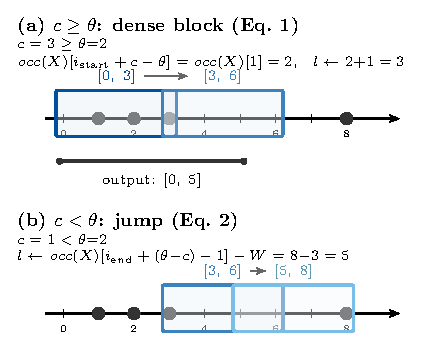
\includegraphics[width=\columnwidth]{scan_stride.pdf}
\caption{Scan Stride Skipping
  (Eqs.~\eqref{eq:stride_dense},~\eqref{eq:stride_sparse}).}
\label{fig:scan_stride}
\end{figure}

\subsection{Apriori Interval Pruning}

The anti-monotonicity of classical Apriori~\cite{agrawal1994fast}
states that every subset of a frequent itemset is also frequent;
equivalently, if any subset is infrequent, its supersets are infrequent.
We apply this property \textit{per interval}.
Since $Y \subseteq X$ implies that every occurrence of $X$ is also an
occurrence of $Y$, for any window $[l, l+W]$:
\[
  \mathrm{sup}(X, l, W) \leq \mathrm{sup}(Y, l, W)
\]
(Lemma~\ref{lem:apriori}, Appendix~C).
Hence if $[l, l+W]$ is not a dense interval for $Y$, it cannot be
one for $X$ either.
For a size-$k$ candidate $X$, the left endpoints $l$ that can be dense
are therefore restricted to the intersection of the dense start-point
sets of all $(k{-}1)$-subsets:
\begin{equation}\label{eq:cand}
  R_X = \bigcap_{Y \subsetneq X,\, |Y|=k-1} \mathcal{T}_\theta(Y),
\end{equation}
where $\mathcal{T}_\theta(Y)$ is the set of left endpoints for which $Y$
is dense.
Any $l \notin R_X$ can safely be skipped, substantially reducing
the scan range.

\subsection{$\Delta$-Step Streaming}

In the target deployment, events arrive continuously from a
sensor stream or autonomous agent log and are appended to a database.
The system triggers a scan every $\Delta$ seconds.

Each scan step proceeds as follows:

\begin{enumerate}
  \item When the $\Delta$-second interval has elapsed (current time $s$),
        retrieve the buffer $[s - W + 1,\; s + \Delta)$, retaining the
        $W{-}1$ most recent events from the previous step to
        prevent boundary loss.
  \item Run the monotone scan with Scan Stride Skipping and
        Apriori Interval Pruning over this buffer, resuming
        from the scan endpoint of the previous step.
  \item Emit all intervals $(X, [l_s, l_e])$ with $l_e + W \leq s$
        not yet output: these are \textbf{confirmed} and will not
        change as future events arrive.
  \item Wait for the next $\Delta$ seconds and repeat.
\end{enumerate}


%%%%%%%%%%%%%%%%%%%%%%%%%%%%%%%%%%%%%%%%%%%%%%%%%%%%
\section{Experiments}\label{sec:experiments}

All experiments were conducted on a single machine
(Apple M3 Pro, 18\,GB RAM) using Rust~1.82 release builds.
To measure \textit{pure computation time} independently of arrival
latency, we pre-load the full dataset and feed it $\Delta$ events
at a time, triggering each scan immediately after the previous completes.

%-----------------------------------------------------------------------
\subsection{EX-1: Scan Frequency Sensitivity}\label{sec:ex1}
%-----------------------------------------------------------------------

We quantify the effect of the scan frequency parameter $\Delta$ on total
processing time and characterize the tradeoff between output latency
and computational cost.
We varied $\Delta \in \{1, 10, 100, 1{,}000, 10{,}000\}$ on a synthetic
stream ($T = 10{,}000$, $|\mathcal{I}| = 20$, $W = 24$, $\theta = 10$;
see Appendix~A for generation details).

\begin{figure}[t]
\centering
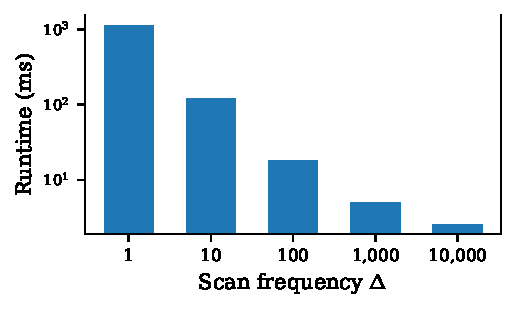
\includegraphics[width=\columnwidth]{ex1_h_vs_time.pdf}
\caption{Scan frequency $\Delta$ vs.\ processing time (log scale).}
\label{fig:ex1}
\end{figure}

As shown in Fig.~\ref{fig:ex1}, each 10$\times$ increase in $\Delta$ reduces
processing time by approximately one order of magnitude, confirming
that reducing scan count directly reduces processing cost.

%-----------------------------------------------------------------------
\subsection{EX-2: Scalability}\label{sec:ex2}
%-----------------------------------------------------------------------

We verify how processing time and peak memory usage scale as stream
length $T$ and item count $|\mathcal{I}|$ are varied independently.
We set $\Delta = T$ (batch mode) and measured pure computation time on
synthetic data ($\theta = 10$, $W = 120$), with baseline
$T = 10^5$ and $|\mathcal{I}| = 24$.

\begin{figure}[t]
\centering
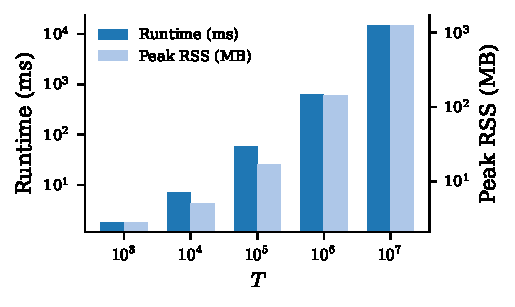
\includegraphics[width=\columnwidth]{ex2_scalability_T.pdf}
\caption{Scalability vs.\ $T$: Runtime and Peak RSS.}
\label{fig:ex2t}
\end{figure}

\begin{figure}[t]
\centering
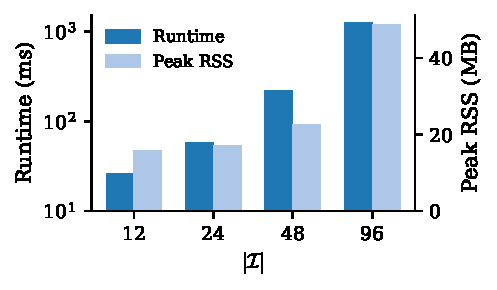
\includegraphics[width=\columnwidth]{ex2_scalability_N.pdf}
\caption{Scalability vs.\ $|\mathcal{I}|$: Runtime and Peak RSS.}
\label{fig:ex2n}
\end{figure}

As shown in Fig.~\ref{fig:ex2t}, runtime scales nearly linearly in $T$
(636\,ms at $T = 10^6$; 15{,}108\,ms at $T = 10^7$).
Fig.~\ref{fig:ex2n} shows super-linear scaling in $|\mathcal{I}|$
(1{,}272\,ms at $|\mathcal{I}| = 96$) due to the combinatorial growth
of higher-order candidates.
Peak RSS scales nearly linearly in $T$ and shows small dependence on
$|\mathcal{I}|$.

%-----------------------------------------------------------------------
\subsection{EX-3: Ablation Study}\label{sec:ex3}
%-----------------------------------------------------------------------

We quantify the independent contributions of Scan Stride Skipping and
Apriori Interval Pruning, and confirm the benefit of combining both.
We set $\Delta = T$ and measured pure computation time on synthetic data
($T = 100{,}000$, $|\mathcal{I}| = 48$, $W = 120$, $\theta = 50$,
epoch overlap 100) for four algorithm variants.

\begin{figure}[t]
\centering
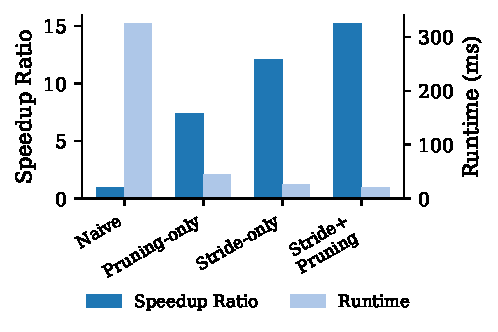
\includegraphics[width=\columnwidth]{ex3_speedup.pdf}
\caption{Ablation: speedup ratio relative to Naive.}
\label{fig:ex3}
\end{figure}

Fig.~\ref{fig:ex3} shows runtime and speedup ratios normalized to
Naive (1.00$\times$).
The Full variant (21.4\,ms) outperforms all individual configurations.
Scan Stride Skipping is the dominant contributor,
achieving a 12.1$\times$ speedup over Naive.
Apriori Interval Pruning alone achieves 7.4$\times$, and combining
both yields 15.2$\times$.
The two techniques contribute independently and complementarily.

%-----------------------------------------------------------------------
\subsection{EX-4: Application to CASAS Sensor Data}\label{sec:ex4}
%-----------------------------------------------------------------------

We apply the algorithm to real sensor streams to confirm that detected
dense intervals correspond to interpretable behavioral routines.
We use two series from the CASAS smart home
dataset~\cite{casas2013} (hh113 and mv001).
CASAS records motion and contact sensor activation streams from
residential environments, structurally analogous to autonomous agent
behavioral logs.
Sensor activations were aggregated into 15-minute time slots.
We set $W = 24$ slots ($= 6$\,hours) to capture activity routines
within specific blocks of the day (morning, evening, or night),
and $\Delta = W = 24$.
Table~\ref{tab:casas_stats} summarizes each dataset.

\begin{table}[t]
\caption{CASAS dataset statistics (slot width $= 15$\,min, $W = 24 = 6$\,h).}
\label{tab:casas_stats}
\begin{center}
\begin{tabular}{ccccc}
\hline
Dataset & $T$ & $|\mathcal{I}|$ & $\theta$ & Patterns \\\hline
hh113 & 48{,}901 & 7 & 14 & 26 \\
mv001 & 139{,}033 & 7 & 18 & 34 \\\hline
\end{tabular}
\end{center}
\end{table}

Representative patterns are listed in
Tables~\ref{tab:casas_hh113} and~\ref{tab:casas_mv001}.
For hh113, the most frequent pattern is the co-occurrence of
DiningRoom and Kitchen (meal preparation/dining), detected across
45 dense intervals.
The co-occurrence of Bathroom and Bedroom (wake/sleep routine)
was found in 8 intervals.
The three-item pattern DiningRoom + Kitchen + OutsideDoor (pre/post-outing
meal behavior) was detected in 7 intervals, showing that the algorithm
captures composite activity transitions.
For mv001, the co-occurrence of Bedroom and LivingRoom
(pre-sleep transition from living room to bedroom) was most frequent
with 113 intervals.
Kitchen and LivingRoom co-occurrence (post-cooking living room stay)
yielded 66 intervals, and the three-item pattern
Bedroom + Kitchen + LivingRoom (full evening-to-bedtime activity chain)
was detected in 44 intervals.

\begin{table}[t]
\caption{Representative detected patterns for hh113.}
\label{tab:casas_hh113}
\begin{center}
\footnotesize
\begin{tabular}{p{3.5cm}cp{2.0cm}}
\hline
Sensor combination & \#Int. & Inferred behavior \\\hline
DiningRoom + Kitchen               & 45 & Meal prep/dining \\
Bathroom + Bedroom                 &  8 & Wake/sleep routine \\
DiningRoom + Kitchen + OutsideDoor &  7 & Pre/post-outing meal \\\hline
\end{tabular}
\end{center}
\end{table}

\begin{table}[t]
\caption{Representative detected patterns for mv001.}
\label{tab:casas_mv001}
\begin{center}
\footnotesize
\begin{tabular}{p{3.5cm}cp{2.0cm}}
\hline
Sensor combination & \#Int. & Inferred behavior \\\hline
Bedroom + LivingRoom               & 113 & Pre-sleep: living$\to$bed \\
Kitchen + LivingRoom               &  66 & Post-cooking living stay \\
Bedroom + Kitchen                  &  44 & Wake/pre-sleep activity \\
Bedroom + Kitchen + LivingRoom     &  44 & Evening-to-bed chain \\\hline
\end{tabular}
\end{center}
\end{table}

The two datasets exhibit distinct behavioral characteristics.
In hh113, food-related patterns dominate, showing that daily routines
centered on the kitchen and dining room repeatedly form within 6-hour
windows.
In mv001, living room-to-bedroom transitions are most frequent,
suggesting that the pre-sleep sequence
(living room $\to$ cooking $\to$ sleep) is an established daily habit.
Bedroom + Office co-occurrence was also detected (23 intervals),
indicating a persistent remote-work pattern.
In both datasets, multi-item patterns ($k \geq 3$) were automatically
enumerated, revealing composite activity transitions not visible
from pairwise co-occurrence alone.
These results demonstrate that Streaming Apriori-Window automatically
detects meaningful behavioral routines from real sensor streams.


%%%%%%%%%%%%%%%%%%%%%%%%%%%%%%%%%%%%%%%%%%%%%%%%%%%%
\section{Conclusion}

We proposed Streaming Apriori-Window, a dense interval mining algorithm
for event streams with an explicit scan frequency parameter $\Delta$.
The confirmed output guarantee follows from the monotone sliding-window
property, ensuring that output intervals are never invalidated by
future events.
Two speedup techniques --- stride-based skipping and Apriori-style
candidate pruning --- reduce processing cost significantly,
with $\Delta = W$ achieving a favorable tradeoff between latency and speed.
Experiments on CASAS smart home sensor data demonstrate that the
algorithm produces interpretable, domain-consistent outputs,
confirming its practical utility for autonomous agent monitoring.

Future work includes applying the framework to behavioral logs from
physical robotic systems, extending it to multi-dimensional event spaces,
and investigating adaptive scan-frequency mechanisms based on
stream characteristics.


%-----------------------------------------------------------------------

\section*{Acknowledgment}
This work is supported by the Honda Bridge Project.
Part of the text in this paper was generated with assistance from Anthropic's large language model Claude~\cite{claude2025}.

%-----------------------------------------------------------------------
%%%%%%%%%%%%%%%%% BIBLIOGRAPHY IN THE LaTeX file !!!!! %%%%%%%%%%%%%%%%%%%%%%

\begin{thebibliography}{99}

\bibitem{takayasu2025arxiv}
K. Takayasu {\it et al.},
``Apriori-Window: Exact enumeration of dense itemset intervals over sliding windows,''
{\it arXiv preprint arXiv:2604.24122}, 2025.

\bibitem{agrawal1994fast}
R. Agrawal and R. Srikant,
``Fast algorithms for mining association rules,''
{\it Proc. VLDB}, pp.~487--499, 1994.

\bibitem{zaki1997new}
M. J. Zaki, S. Parthasarathy, M. Ogihara, and W. Li,
``New algorithms for fast discovery of association rules,''
{\it Proc. KDD}, pp.~283--296, 1997.

\bibitem{han2000mining}
J. Han, J. Pei, and Y. Yin,
``Mining frequent patterns without candidate generation,''
{\it ACM SIGMOD Record}, vol.~29, no.~2, pp.~1--12, 2000.

\bibitem{fournier2017survey}
P. Fournier-Viger, J. C.-W. Lin, B. Vo, T. T. Chi, J. Zhang, and H. B. Le,
``A survey of itemset mining,''
{\it WIREs Data Mining Knowl. Discov.}, vol.~7, no.~4, e1207, 2017.

\bibitem{yin2014lpfim}
K.-C. Yin, Y.-L. Hsieh, D.-L. Yang, and M.-C. Hung,
``Association rule mining considering local frequent patterns with temporal intervals,''
{\it Applied Mathematics \& Information Sciences}, vol.~8, no.~4,
pp.~1879--1890, 2014.

\bibitem{saleh2011lppm}
B. Saleh and F. Masseglia,
``Discovering frequent behaviors: Time is an essential element of the context,''
{\it Knowledge and Information Systems}, vol.~28, no.~2, pp.~311--331, 2011.

\bibitem{kiran2017rpm}
R. U. Kiran, J. Venkatesh, M. Toyoda, M. Kitsuregawa, and P. K. Reddy,
``Discovering partial periodic-frequent patterns in a transactional database,''
{\it J. Systems and Software}, vol.~125, pp.~170--182, 2017.

\bibitem{fournierviger2021glf}
P. Fournier-Viger {\it et al.},
``Mining local periodic patterns in a discrete sequence,''
{\it Information Sciences}, vol.~544, pp.~519--548, 2021.

\bibitem{kiran2015sim}
R. U. Kiran, H. Shang, M. Toyoda, and M. Kitsuregawa,
``Discovering recurring patterns in time series,''
{\it Proc. EDBT}, pp.~97--108, 2015.

\bibitem{lee2001sliding}
C.-H. Lee, C.-R. Lin, and M.-S. Chen,
``Sliding-window filtering: An efficient algorithm for incremental mining,''
{\it Proc. CIKM}, pp.~263--270, 2001.

\bibitem{leung2006dstree}
C. K.-S. Leung and Q. I. Khan,
``DSTree: A tree structure for the mining of frequent sets from data streams,''
{\it Proc. ICDM}, pp.~928--932, 2006.

\bibitem{luna2019fim}
J. M. Luna {\it et al.},
``Frequent itemset mining: A 25 years review,''
{\it WIREs Data Mining Knowl. Discov.}, vol.~9, no.~6, e1320, 2019.

\bibitem{fournierviger2022survey}
P. Fournier-Viger {\it et al.},
``Pattern mining: Current challenges and opportunities,''
{\it Proc. DASFAA Workshops}, pp.~3--19, 2022.

\bibitem{liu1999multiple}
B. Liu, W. Hsu, and Y. Ma,
``Mining association rules with multiple minimum supports,''
{\it Proc. KDD}, pp.~337--341, 1999.

\bibitem{tanbeer2009pfpm}
S. K. Tanbeer, C. F. Ahmed, B.-S. Jeong, and Y.-K. Lee,
``Discovering periodic-frequent patterns in transactional databases,''
{\it Proc. PAKDD}, pp.~242--253, 2009.

\bibitem{kleinberg2003bursty}
J. Kleinberg,
``Bursty and hierarchical structure in streams,''
{\it Data Mining Knowl. Discov.}, vol.~7, no.~4, pp.~373--397, 2003.

\bibitem{yang2021burstsketch}
Z. Zhong, S. Yan, Z. Li, D. Tan, T. Yang, and B. Cui,
``BurstSketch: Finding bursts in data streams,''
{\it Proc. ACM SIGMOD}, pp.~2375--2383, 2021.

\bibitem{casas2013}
D. J. Cook, A. S. Crandall, B. L. Thomas, and N. C. Krishnan,
``CASAS: A smart home in a box,''
{\it IEEE Computer}, vol.~46, no.~7, pp.~62--69, 2013.

\bibitem{claude2025}
Anthropic,
``Claude,'' Anthropic, \url{https://www.anthropic.com/claude} (accessed 2026-10-28).

\end{thebibliography}

%%%%%%%%%%%%%%%%%%%%%%%%%%%%%%%%%%%%%%%%%%%%%%%%%%%%
\appendix

\section{Synthetic Data Generation}

Synthetic streams are generated with epoch-structured item occurrence patterns.

\textbf{Epoch structure.}
Each of the $|\mathcal{I}|$ items $i = 0, 1, \ldots, |\mathcal{I}|{-}1$
is assigned a dense epoch within the stream.
The epoch width is
\[
  L_{\mathrm{ep}} = \left\lfloor \frac{T}{|\mathcal{I}|} \right\rfloor \times 3,
\]
with step width $\mathrm{step} = L_{\mathrm{ep}} - 2$ so that epochs of
adjacent items overlap by two items.
Item $i$ starts its epoch at $s_i = (i \times \mathrm{step}) \bmod T$,
giving the epoch interval $[s_i,\; s_i + L_{\mathrm{ep}})$
(with wraparound at boundary).

\textbf{Firing probability.}
At each timestep $t$, item $i$ appears in the stream with probability
\[
  p_i(t) =
  \begin{cases}
    0.8  & t \text{ is within item } i\text{'s epoch} \\
    0.05 & \text{otherwise}
  \end{cases}
\]
Each item is sampled independently.

%-----------------------------------------------------------------------
\section{Validity of Scan Stride Skipping}

\begin{lemma}[Validity of Dense Phase]\label{lem:stride_dense}
In window $[l, l+W]$ let $c = \mathrm{sup}(X, l, W) \geq \theta$,
and set $l_{\mathrm{dense}} = \mathit{occ}(X)[i_{\mathrm{start}} + c - \theta]$.
Then for every $l' \in [l,\, l_{\mathrm{dense}}]$,
$\mathrm{sup}(X, l', W) \geq \theta$.
\end{lemma}

\begin{proof}
Let the occurrences in $[l, l+W]$ be
$\mathit{occ}(X)[i_{\mathrm{start}}], \ldots, \mathit{occ}(X)[i_{\mathrm{start}}+c-1]$.
For $l' \leq l_{\mathrm{dense}} = \mathit{occ}(X)[i_{\mathrm{start}}+c-\theta]$,
the $\theta$ occurrences
$\mathit{occ}(X)[i_{\mathrm{start}}+c-\theta], \ldots, \mathit{occ}(X)[i_{\mathrm{start}}+c-1]$
all lie in $[l', l'+W]$:
lower bound $\mathit{occ}(X)[i_{\mathrm{start}}+c-\theta] \geq l'$ (by assumption);
upper bound $\mathit{occ}(X)[i_{\mathrm{start}}+c-1] \leq l+W \leq l'+W$ (since $l \leq l'$).
Hence $\mathrm{sup}(X, l', W) \geq \theta$.
\end{proof}

\begin{lemma}[Validity of Non-Dense Phase]\label{lem:stride_sparse}
In window $[l, l+W]$ let $c = \mathrm{sup}(X, l, W) < \theta$,
and set $l_{\mathrm{new}} = \mathit{occ}(X)[i_{\mathrm{end}} + (\theta-c) - 1] - W$.
Then for every $l' \in (l,\, l_{\mathrm{new}})$,
$\mathrm{sup}(X, l', W) < \theta$.
\end{lemma}

\begin{proof}
Partition the occurrences in $[l', l'+W]$ into two parts.
(i)~In $[l', l+W] \subseteq [l, l+W]$: at most $c$ occurrences.
(ii)~In $(l+W, l'+W]$: since $l' < l_{\mathrm{new}}$ we have
$l'+W < \mathit{occ}(X)[i_{\mathrm{end}}+(\theta-c)-1]$,
so this part contains occurrences
$\mathit{occ}(X)[i_{\mathrm{end}}], \ldots, \mathit{occ}(X)[i_{\mathrm{end}}+(\theta-c)-2]$,
at most $\theta-c-1$.
Total $\leq c + (\theta-c-1) = \theta - 1 < \theta$.
\end{proof}

%-----------------------------------------------------------------------
\section{Validity of Apriori Interval Pruning}

\begin{lemma}[Candidate Range Restriction by Anti-Monotonicity]\label{lem:apriori}
For an itemset $X$ of size $k$, if some $(k{-}1)$-subset $Y \subsetneq X$
satisfies $\mathrm{sup}(Y, l, W) < \theta$ in window $[l, l+W]$,
then $\mathrm{sup}(X, l, W) < \theta$.
\end{lemma}

\begin{proof}
If $X \subseteq I_t$ then $Y \subset X \subseteq I_t$, so
$\{t \in \mathit{occ}(X) : l \leq t \leq l+W\} \subseteq
 \{t \in \mathit{occ}(Y) : l \leq t \leq l+W\}$.
Hence $\mathrm{sup}(X, l, W) \leq \mathrm{sup}(Y, l, W) < \theta$.
\end{proof}

By Lemma~\ref{lem:apriori}, any $l$ not in the intersection
$R_X = \bigcap_{Y \subsetneq X,\, |Y|=k-1} \mathcal{T}_\theta(Y)$
cannot yield a dense window for $X$, so scanning $R_X$ alone suffices.



\end{document}
